\documentclass[17pt]{beamer} %Makes presentation
%\documentclass[handout]{beamer} %Makes Handouts
\usetheme{Singapore} %Gray with fade at top
\useoutertheme[subsection=false]{miniframes} %Supppress subsection in header
\useinnertheme{rectangles} %Itemize/Enumerate boxes
\usecolortheme{seagull} %Color theme
\usecolortheme{rose} %Inner color theme

\definecolor{light-gray}{gray}{0.75}
\definecolor{dark-gray}{gray}{0.55}
\setbeamercolor{item}{fg=light-gray}
\setbeamercolor{enumerate item}{fg=dark-gray}

\setbeamertemplate{navigation symbols}{}
%\setbeamertemplate{mini frames}[default]
%\setbeamercovered{dynamics}
\setbeamerfont*{title}{size=\Large,series=\bfseries}
\setbeamerfont{footnote}{size=\tiny}

%\setbeameroption{notes on second screen} %Dual-Screen Notes
%\setbeameroption{show only notes} %Notes Output

\setbeamertemplate{frametitle}{\vspace{.5em}\bfseries\insertframetitle}
\newcommand{\heading}[1]{\noindent \textbf{#1}\\ \vspace{1em}}

\usepackage{bbding,color,multirow,times,ccaption,tabularx,graphicx,verbatim,booktabs}
\usepackage{colortbl} %Table overlays
\usepackage[english]{babel}
%\usepackage[latin1]{inputenc}
%\usepackage[T1]{fontenc}
\usepackage{lmodern}

%\author[]{Thomas J. Leeper}
\institute[]{
  \inst{}%
  Department of Government\\London School of Economics and Political Science
}

\usepackage{tikz}
\usetikzlibrary{shapes,arrows}

\title{Getting to Regression: The Workhorse of Quantitative Political Analysis}


\date[]{}

\begin{document}

\frame{\titlepage}

\frame{\tableofcontents}

\section[Review]{Simple Statistics}
\frame{\tableofcontents[currentsection]}


\frame{
\frametitle{Relationship}

\begin{itemize}\itemsep1em
\item<1-> Covariance:\\
	$Cov(X,Y) = \sum_{i=1}^{n} \dfrac{(X_i - \bar{X})(Y_i - \bar{Y})}{n-1}$
\item<2-> Correlation:\\
	{\small $Corr(X,Y) = r_{x,y} = \sum_{i=1}^{n} \dfrac{(X_i - \bar{X})(Y_i - \bar{Y})}{(n-1)s_x s_y}$}
\end{itemize}
}


\frame{

\frametitle{Correlation is linear!}

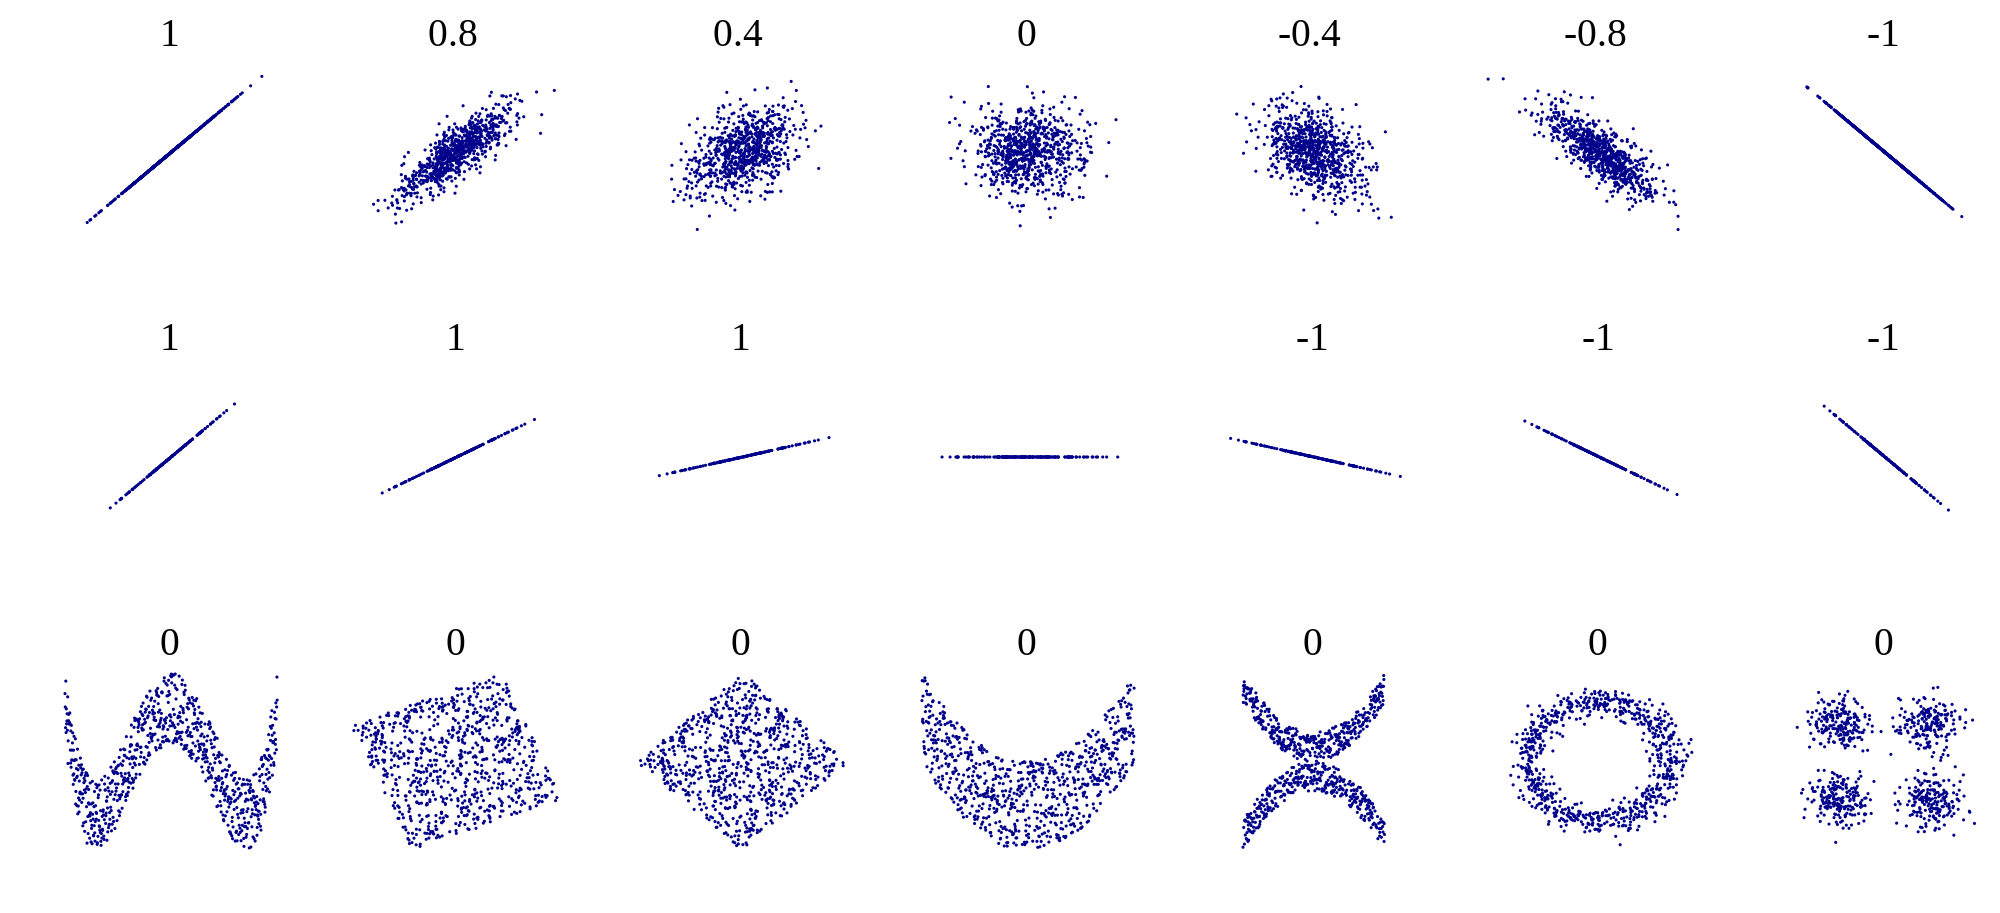
\includegraphics[width=\textwidth]{images/correlation}

\vspace{1em}
{\footnotesize Source: \href{https://commons.wikimedia.org/wiki/File:Correlation_examples2.svg}{Wikimedia}}
}

\frame{
	\frametitle{Guess the Correlation!}
	\begin{enumerate}\itemsep0.5em
	\item Go to: {\small \url{http://guessthecorrelation.com/}}
	\item Play a few rounds
	\end{enumerate}

}



\end{document}
